% KubeFinOps paper draft (IEEE conference format).
% Build: latexmk -pdf main.tex   (or upload the paper/ folder to Overleaf, which ships IEEEtran)
% Tables in generated/ and figures in figures/ are produced by:
%   python -m kfo_research.experiments            (from research/)
\documentclass[conference]{IEEEtran}
\usepackage{amsmath,amssymb}
\usepackage{graphicx}
\usepackage{booktabs}
\usepackage{url}
\usepackage[hidelinks]{hyperref}
\usepackage{xcolor}
\newcommand{\todo}[1]{\textcolor{red}{[TODO: #1]}}
\graphicspath{{figures/}}

\begin{document}

\title{SLO-Aware Right-Sizing for Kubernetes:\\Cost Savings Without Breaking Workloads}

\author{
\IEEEauthorblockN{\todo{Author 1}, \todo{Author 2}, \todo{Author 3}, \todo{Author 4}}
\IEEEauthorblockA{\todo{Department, Institute}\\\todo{emails}}
}

\maketitle

\begin{abstract}
Kubernetes clusters are routinely provisioned for peaks that never come: containers request several times
the CPU and memory they use, and the unreserved remainder of every node is paid for but idle. Right-sizing
tools close this gap by recomputing resource requests from observed usage, but popular rules---a high
percentile plus a fixed margin, or the Vertical Pod Autoscaler's histogram estimator---optimise for savings and
leave the resulting reliability risk implicit. We present an \emph{SLO-aware} right-sizing method that makes the
risk explicit and tunable: the CPU request is the smallest value whose \emph{peak} demand is exceeded in at most
an $\varepsilon$ share of (recency-weighted) time, with headroom derived from the day-to-day variability of the
daily peak; observations clipped by a CPU limit are treated as censored, out-of-memory kills as evidence that
demand exceeds the limit, and sustained memory growth blocks reductions. The method runs inside KubeFinOps, an
open-source FinOps platform that allocates cost with the OpenCost model, detects waste, and applies changes
through a dry-run, two-person approval and automatic-rollback workflow. In a trace-driven evaluation on 200
containers spanning eight workload archetypes, the method saved 41.4\% of requested cost while keeping CPU
under-provisioning at 0.47\% of windows (target $\varepsilon = 1\%$) with no OOM events, versus 55.1\% / 11.4\% for
p95+20\% and 63.9\% / 18.8\% with 67 OOM events for a VPA-style estimator. On 2,037 production containers
from Alibaba cluster-trace-v2018 it saved 63.8\% at 0.39\% CPU under-provisioning, versus 77.5\% / 3.2\% and
80.0\% / 7.9\%, and pushed memory below observed use in fewer containers (28 vs.\ 38 and 69).
\end{abstract}

\begin{IEEEkeywords}
Kubernetes, FinOps, right-sizing, resource management, cloud cost, service-level objectives
\end{IEEEkeywords}

\section{Introduction}
Container orchestration made it easy to run many services on shared clusters, but the resource requests that
drive scheduling---and therefore cost---are set by developers who rarely know their workload's true needs.
Analyses of production traces consistently report low utilisation of reserved capacity~\cite{guo2019alibaba,
tirmazi2020borg,cortez2017resourcecentral}. Because cloud providers bill whole nodes, every core requested but
unused is money spent; the FinOps practice~\cite{finopsfoundation} aims to make this spend visible and actionable.

Right-sizing tools recommend smaller (or larger) requests from observed usage. Two designs dominate practice: a
fixed rule such as ``95th percentile of usage plus 20\%'', and the Kubernetes Vertical Pod Autoscaler
(VPA)~\cite{k8svpa}, which keeps decaying histograms of usage and targets their 90th percentile plus a 15\% margin,
inspired by Autopilot~\cite{rzadca2020autopilot}. Both choose a savings level and leave the reliability
consequence implicit; neither distinguishes compressible CPU (contention degrades latency) from incompressible
memory (exceeding the limit kills the container), and neither accounts for measurements distorted by the very
limits being tuned.

\textbf{Contributions.} (1) An SLO-aware right-sizing method whose single parameter $\varepsilon$ is the tolerated
share of time in which peak CPU demand exceeds the request (Section~\ref{sec:method}), with three corrections:
day-to-day peak variability as headroom, censoring-aware estimation when CPU is throttled at a limit, and
OOM/leak-aware memory sizing. (2) KubeFinOps, an open-source platform that implements the method end to end:
OpenCost-compatible allocation, waste detection, and a guarded remediation loop (Section~\ref{sec:system}).
(3) A trace-driven evaluation with an interactive replay simulator that feeds OOM events and changed limits back
into the history, comparing the method with p95+20\% and a faithful VPA-style estimator
(Section~\ref{sec:eval}).

\section{Background and Related Work}
\textbf{Cluster resource management.} Borg~\cite{verma2015borg} and its successors~\cite{burns2016borg} introduced
request-based scheduling and overcommitment; Autopilot~\cite{rzadca2020autopilot} showed that automated vertical
scaling at Google cut slack substantially while keeping out-of-memory events rare. Quasar~\cite{delimitrou2014quasar}
and Resource Central~\cite{cortez2017resourcecentral} use learned models to predict resource needs. Kubernetes'
VPA~\cite{k8svpa} brings a histogram-based recommender to open-source clusters.

\textbf{Cost allocation.} OpenCost~\cite{opencost} defines how to attribute node cost to containers: a container
pays for the larger of its request and its usage at the node's unit prices; unreserved capacity is idle cost.
KubeFinOps follows this model so that savings are measured in the currency finance teams use.

\textbf{Gap.} Existing recommenders expose margins and percentiles, not a service-level target, and treat CPU and
memory symmetrically. We make the reliability target the input, and correct for censored and fatal observations.

\section{SLO-Aware Right-Sizing}\label{sec:method}
For one container (replicas pooled), let window $i$ (5 minutes) have mean CPU $c_i$, peak CPU $\hat c_i$, peak
working set $\hat m_i$, throttled seconds $\theta_i$ and OOM kills $k_i$, with recency weight
$w_i = \Delta_i \, 2^{-(t_{\max}-t_i)/h}$ (half-life $h = 48$\,h).

\textbf{CPU.} The request is
\begin{equation}
r_{\mathrm{cpu}} = Q^{w}_{1-\varepsilon}\big(\{\hat c_i\}\big)\cdot\big(1 + \min(\eta, \kappa\,\mathrm{CV}_{\mathrm{day}})\big),
\end{equation}
where $Q^w_q$ is the weighted $q$-quantile of \emph{peaks} and $\mathrm{CV}_{\mathrm{day}}$ is the coefficient of
variation of the daily maximum over complete days. Using peaks rather than means targets contention directly;
using day-to-day peak variability (rather than the CV of all samples) protects against the next peak exceeding
past ones without penalising on/off batch jobs whose nightly peak never changes.

\textbf{Censoring.} When a CPU limit $\ell$ is set and the throttled share
$\rho = \sum\theta_i / \sum\Delta_i$ exceeds a threshold, observed peaks are clipped and under-state demand. We
lift the estimate above the observed clipping level $L = \max_i \hat c_i$:
$r_{\mathrm{cpu}} \leftarrow \max\big(r_{\mathrm{cpu}}, \min(L(1+\rho), \gamma\max(r, L))\big)$, with $\gamma = 2$
bounding a single step. Anchoring on $L$---not on the current limit---matters: anchoring on the limit made the
estimate compound on every run while old throttled samples remained in the window, a failure our replay exposed.

\textbf{Memory.} Memory is incompressible, so we size from the maximum peak working set plus headroom
$\beta + \lambda\,\mathrm{CV}_m$. Each OOM kill is a censored observation of demand $\geq$ the limit and raises the
request above it; sustained growth of hourly maxima (leak signature) adds a projection and blocks reductions.
Memory limit equals request.

\textbf{Safety.} Reductions are capped at 50\% per step and re-evaluated after verification; each recommendation
carries a confidence (history length $\times$ completeness) and a risk label. HPA-managed workloads keep the
request high enough not to trigger scale-out.

\section{The KubeFinOps Platform}\label{sec:system}
An in-cluster agent with read-only RBAC reads inventory from the Kubernetes API and per-container usage from
Prometheus (cAdvisor and kube-state-metrics) every five minutes, including CPU throttling (CFS periods), restarts
and OOM kills, and pushes them to a central server backed by TimescaleDB. The server allocates cost per hour with
the OpenCost model using node prices from AWS, GCP and Azure catalogs, detects waste (idle workloads, orphaned
volumes, load balancers without endpoints, consolidatable nodes), forecasts spend with Holt-Winters~\cite{winters1960forecasting}
and flags cost anomalies with a robust z-score~\cite{rousseeuw1993mad} of forecast errors.

Changes are never applied blindly: a proposed change is first \emph{dry-run} on the cluster's API server,
approved by a second operator, applied inside a change window, and watched; if OOM kills, restarts or throttling
rise compared with the period before the change, an automatic rollback restores the captured specification. All
steps are written to a hash-chained audit log (Fig.~\ref{fig:arch}).

\begin{figure*}[t]
\centering
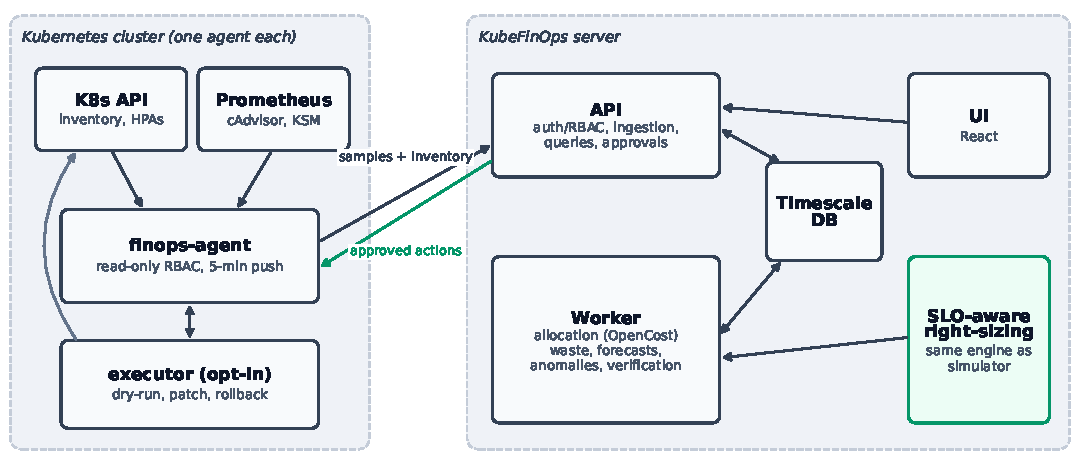
\includegraphics[width=0.85\textwidth]{architecture.pdf}
\caption{KubeFinOps architecture. Agents push data out of each cluster, so the server needs no access to
cluster API servers; the right-sizing engine evaluated in this paper is the one the worker runs.}
\label{fig:arch}
\end{figure*}

\section{Evaluation}\label{sec:eval}
\textbf{Replay simulator.} For each container and strategy, after a 7-day warm-up the strategy is re-run daily on
a 14-day rolling window and its requests apply to the next day, starting from the developer's original requests.
Memory peaks above the request count as OOM events and are fed back into the history; for traces clipped by a CPU
limit, the history is re-observed under the limit in force (a raised limit stops throttling), and
under-provisioning is measured against the true demand. Cost uses OpenCost default unit prices.

\textbf{Workloads.} 200 synthetic containers (25 per archetype, 21 days, fixed seed): diurnal web services,
spiky APIs, nightly batch jobs, memory leaks, CPU-capped services, growing services, idle and under-provisioned
containers. Original requests follow common practice (1.5--4$\times$ observed peaks; some below need).
For real-trace validation we use Alibaba cluster-trace-v2018~\cite{alibabatrace2018} (Section~\ref{sec:alibaba}).

\textbf{Metrics.} Cost savings versus original requests; share of windows whose true CPU peak exceeds the request
(\emph{CPU under}); CPU deficit (core-hours of demand above the request, relative to requested core-hours); OOM
events and containers affected.

\begin{table}[t]
\centering
\caption{Overall results (200 containers, 14 evaluated days each).}
\label{tab:main}
\resizebox{\columnwidth}{!}{\begin{tabular}{lrrrrr}\toprule
Strategy & Savings (\%) & CPU under (\%) & CPU deficit (\%) & OOM events & Containers w/ OOM \\\midrule
Original requests & 0.0 & 9.40 & 0.77 & 0 & 0 \\
p95 + 20\% & 55.1 & 11.39 & 1.14 & 0 & 0 \\
VPA-style & 63.9 & 18.77 & 4.63 & 67 & 2 \\
SLO-aware (ours) & 41.4 & 0.47 & 0.03 & 0 & 0 \\
\bottomrule\end{tabular}
}
\end{table}

\begin{figure}[t]
\centering
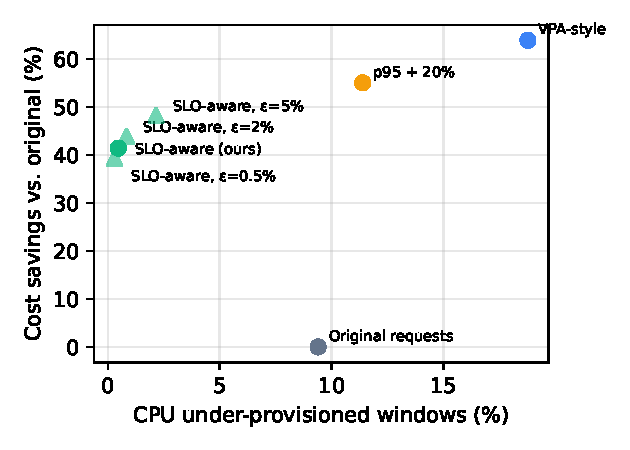
\includegraphics[width=\columnwidth]{pareto_synthetic.pdf}
\caption{Savings vs.\ CPU under-provisioning. The SLO-aware method traces a tunable frontier through
$\varepsilon$; realised under-provisioning stays below the target.}
\label{fig:pareto}
\end{figure}

\textbf{Results.} Table~\ref{tab:main} and Fig.~\ref{fig:pareto}: the SLO-aware method saves 41.4\% while
keeping CPU under-provisioning at 0.47\% of windows and causing no OOM events; p95+20\% saves 55.1\% at 11.4\%
under-provisioning; the VPA-style estimator saves 63.9\% at 18.8\% and 67 OOM events, all on memory-leaking
containers. Across $\varepsilon \in \{0.5, 1, 2, 5\}\%$ the realised rate (0.30, 0.47, 0.83, 2.15\%) stays below
the target while savings rise from 39.3\% to 48.3\%, so $\varepsilon$ is an honest operating knob.

\begin{table}[t]
\centering
\caption{Ablation and $\varepsilon$ sweep.}
\label{tab:ablation}
\resizebox{\columnwidth}{!}{\begin{tabular}{lrrrrr}\toprule
Strategy & Savings (\%) & CPU under (\%) & CPU deficit (\%) & OOM events & Containers w/ OOM \\\midrule
SLO-aware (ours) & 41.4 & 0.47 & 0.03 & 0 & 0 \\
-- censoring correction & 41.7 & 0.61 & 0.05 & 0 & 0 \\
-- OOM feedback & 41.4 & 0.47 & 0.03 & 0 & 0 \\
-- recency weighting & 41.9 & 0.53 & 0.04 & 0 & 0 \\
-- daily-peak headroom & 46.0 & 1.37 & 0.12 & 0 & 0 \\
-- step cap (one-shot) & 42.6 & 0.54 & 0.04 & 0 & 0 \\
SLO-aware, $\varepsilon$=0.5\% & 39.3 & 0.30 & 0.02 & 0 & 0 \\
SLO-aware, $\varepsilon$=2\% & 44.0 & 0.83 & 0.06 & 0 & 0 \\
SLO-aware, $\varepsilon$=5\% & 48.3 & 2.15 & 0.27 & 0 & 0 \\
\bottomrule\end{tabular}
}
\end{table}

\textbf{Ablation} (Table~\ref{tab:ablation}). Removing daily-peak headroom raises under-provisioning from 0.47\% to
1.37\%; removing the censoring correction nearly doubles it on CPU-capped services (1.32\% $\rightarrow$ 2.50\%,
Table~\ref{tab:arch}); the 50\% step cap costs only 1.2 points of savings. Recency weighting and OOM feedback did not
change outcomes on these stationary traces (no OOM occurred under the method); we expect them to matter on
non-stationary real workloads.

\begin{table*}[t]
\centering
\caption{Per archetype: savings (\%) and CPU under-provisioning (\%) / OOM events.}
\label{tab:arch}
\begin{tabular}{lrrrrrr}\toprule
 & \multicolumn{2}{c}{p95+20\%} & \multicolumn{2}{c}{VPA-style} & \multicolumn{2}{c}{SLO-aware} \\
Archetype & Sav.\% & Under\% / OOM & Sav.\% & Under\% / OOM & Sav.\% & Under\% / OOM \\\midrule
batch nightly & 25 & 0.0 / 0 & 62 & 6.9 / 0 & 24 & 0.6 / 0 \\
cpu capped & 13 & 7.3 / 0 & 17 & 12.5 / 0 & -17 & 1.3 / 0 \\
growing & 72 & 18.9 / 0 & 72 & 19.0 / 0 & 58 & 0.4 / 0 \\
idle & 97 & 17.1 / 0 & 95 & 0.1 / 0 & 91 & 0.2 / 0 \\
memory leak & 56 & 22.8 / 0 & 57 & 50.8 / 67 & 45 & 0.4 / 0 \\
spiky api & 76 & 15.0 / 0 & 82 & 33.0 / 0 & 46 & 0.5 / 0 \\
under provisioned & -27 & 4.8 / 0 & -15 & 13.8 / 0 & -57 & 0.2 / 0 \\
web diurnal & 70 & 5.1 / 0 & 73 & 14.0 / 0 & 61 & 0.1 / 0 \\
\bottomrule\end{tabular}

\end{table*}

\subsection{Production traces (Alibaba v2018)}\label{sec:alibaba}
\textbf{Data.} The container usage table is $\approx$29\,GB compressed; we stream its first 300\,MB (40,075
containers, median span 8 days) and evaluate a deterministic 5\% hash sample of the containers with at least
7.5 days of data and 60\% coverage (2,037 containers, median request 4 cores). Samples are sparse, so windows
are 15 minutes (mean and peak). CPU utilisation is relative to the request: the observed peak never exceeds it
(median peak/request 0.30, p95 0.81), consistent with limit $=$ request. Memory utilisation is relative to the
container's memory size and includes page cache: 70\% of containers reach their size, and some exceed it
without being killed. We therefore treat the original memory allocation as known-safe: a memory event is
counted only when a strategy lowered the limit \emph{below} the original and the observed peak exceeds it.
With an 8-day span we use a 3-day warm-up, so each container is evaluated for about 5 days.

\begin{table}[t]
\centering
\caption{Alibaba v2018, 2,037 containers. ``OOM'' counts windows whose memory exceeded a limit lowered below
the original.}
\label{tab:alibaba}
\resizebox{\columnwidth}{!}{\begin{tabular}{lrrrrr}\toprule
Strategy & Savings (\%) & CPU under (\%) & CPU deficit (\%) & OOM events & Containers w/ OOM \\\midrule
Original requests & 0.0 & 0.00 & 0.00 & 0 & 0 \\
p95 + 20\% & 77.5 & 3.20 & 0.79 & 1222 & 38 \\
VPA-style & 80.0 & 7.92 & 1.61 & 2498 & 69 \\
SLO-aware (ours) & 63.8 & 0.39 & 0.11 & 582 & 28 \\
\bottomrule\end{tabular}
}
\end{table}

\begin{figure}[t]
\centering
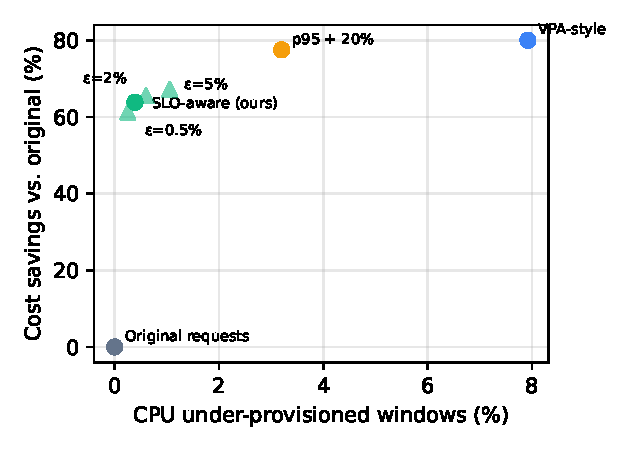
\includegraphics[width=\columnwidth]{pareto_alibaba.pdf}
\caption{Alibaba v2018: savings vs.\ CPU under-provisioning, including the $\varepsilon$ sweep.}
\label{fig:pareto-alibaba}
\end{figure}

\textbf{Results} (Table~\ref{tab:alibaba}, Fig.~\ref{fig:pareto-alibaba}). Production containers are far more
over-provisioned than our synthetic ones, so all strategies save more. The SLO-aware method saves 63.8\% at
0.39\% CPU under-provisioning; p95+20\% saves 77.5\% but under-provisions 8$\times$ as often (3.2\%) and VPA-style
80.0\% at 20$\times$ (7.9\%), with CPU deficits of 0.79\% and 1.61\% vs.\ 0.11\%. The calibration seen on
synthetic data holds: for $\varepsilon \in \{0.5, 1, 2, 5\}\%$ the realised rate is 0.25, 0.39, 0.60 and 1.05\%,
always below the target. Memory events touch 28 containers (1.4\%) under the method versus 38 and 69 for the
baselines. We did not tune the method for this trace, and with only a 3-day warm-up the memory history is
short; longer traces are needed to tell how much of this residual risk remains.

\begin{table}[t]
\centering
\caption{Alibaba v2018: ablation and $\varepsilon$ sweep.}
\label{tab:ablation-alibaba}
\resizebox{\columnwidth}{!}{\begin{tabular}{lrrrrr}\toprule
Strategy & Savings (\%) & CPU under (\%) & CPU deficit (\%) & OOM events & Containers w/ OOM \\\midrule
SLO-aware (ours) & 63.8 & 0.39 & 0.11 & 582 & 28 \\
-- censoring correction & 63.8 & 0.39 & 0.11 & 582 & 28 \\
-- OOM feedback & 63.9 & 0.39 & 0.11 & 582 & 28 \\
-- recency weighting & 63.8 & 0.40 & 0.12 & 583 & 28 \\
-- daily-peak headroom & 66.8 & 1.01 & 0.22 & 545 & 27 \\
-- step cap (one-shot) & 71.5 & 0.56 & 0.19 & 711 & 36 \\
SLO-aware, $\varepsilon$=0.5\% & 61.2 & 0.25 & 0.08 & 557 & 29 \\
SLO-aware, $\varepsilon$=2\% & 65.5 & 0.60 & 0.17 & 582 & 28 \\
SLO-aware, $\varepsilon$=5\% & 67.2 & 1.05 & 0.28 & 545 & 27 \\
\bottomrule\end{tabular}
}
\end{table}

\textbf{Ablation on real traces} (Table~\ref{tab:ablation-alibaba}). Daily-peak headroom is again the main
protection (0.39\% $\rightarrow$ 1.01\% without it), and the step cap now matters more: a one-shot reduction
raises memory events from 28 to 36 containers. The censoring correction has no effect because no container is
pinned at its CPU limit in this sample, and OOM feedback and recency weighting hardly matter over 5 evaluated
days.

\textbf{Threats to validity.} Synthetic archetypes are our own design. The Alibaba sample covers the head of
the usage file (one week) and memory utilisation includes page cache, so memory results are indicative only.
The replay cannot model contention between containers on a node, and treats CPU exceedance as risk rather
than measured latency.

\section{Conclusion}
Making the reliability target the input of right-sizing turns a savings knob into an SLO: in our evaluation the
method kept CPU under-provisioning below its target and avoided all OOM events while still removing 41\% of
requested cost, and on 2,037 Alibaba production containers it removed 64\% at 0.39\% under-provisioning, 8--20$\times$
less than the p95 and VPA-style baselines. KubeFinOps packages the method with cost allocation, waste detection and a guarded remediation
loop; code, traces and the replay simulator are open source.

\bibliographystyle{IEEEtran}
\bibliography{refs}

\end{document}
